\documentclass[12pt, spanish]{article}
\usepackage[spanish]{babel}
\selectlanguage{spanish}
\usepackage{natbib}
\usepackage{url}
\usepackage[utf8x]{inputenc}
\usepackage{graphicx}
\graphicspath{{images/}}
\usepackage{parskip}
\usepackage{fancyhdr}
\usepackage{vmargin}

\usepackage{hyperref}
\usepackage[
    type={CC},
    modifier={by-nc-sa},
    version={4.0},
]{doclicense}

\hypersetup{
    colorlinks=true,
    linkcolor=blue,
    filecolor=magenta,      
    urlcolor=cyan,
}

\usepackage[default]{sourcesanspro}

\setmarginsrb{2 cm}{1 cm}{2 cm}{2 cm}{1 cm}{1.5 cm}{1 cm}{1.5 cm}

\title{Modelos de Computación:\\
Práctica 3. \hspace{0.05cm} }                           
\author{Antonio David Villegas Yeguas}                             
\date{\today}                                           

\renewcommand*\contentsname{hola}

\makeatletter
\let\thetitle\@title
\let\theauthor\@author
\let\thedate\@date
\makeatother

\pagestyle{fancy}
\fancyhf{}
\rhead{\theauthor}
\lhead{\thetitle}
\cfoot{\thepage}

\begin{document}
%%%%%%%%%%%%%%%%%%%%%%%%%%%%%%%%%%%%%%%%%%%%%%%%%%%%%%%%%%%%%%%%%%%%%%%%%%%%%%%%%%%%%%%%%

\begin{titlepage}
    \centering
    \vspace*{0.5 cm}
    
\includegraphics[scale = 0.50]{ugr.png}\\[1.0 cm]
    %\textsc{\LARGE Universidad de Granada}\\[2.0 cm]   
    \textsc{\large 3ºA - A2}\\[0.5 cm]            
    \textsc{\large Grado en Ingeniería Informática}\\[0.5 cm]              
    \rule{\linewidth}{0.2 mm} \\[0.2 cm]
    { \huge \bfseries \thetitle}\\
    \rule{\linewidth}{0.2 mm} \\[1 cm]
    
    \begin{minipage}{0.4\textwidth}
        \begin{flushleft} \large
            \emph{Autor:}\\
            \theauthor
            \end{flushleft}
            \end{minipage}~
            \begin{minipage}{0.4\textwidth}
            \begin{flushright} \large
            \emph{Asignatura: \\
            Modelos de Computación}                   
        \end{flushright}
    \end{minipage}\\[0.5cm]
  
    {\large \thedate}\\[0.5cm]
    {\url{https://github.com/advy99/MC/}}
    {\doclicenseThis}
 	
    \vfill
    
\end{titlepage}

%%%%%%%%%%%%%%%%%%%%%%%%%%%%%%%%%%%%%%%%%%%%%%%%%%%%%%%%%%%%%%%%%%%%%%%%%%%%%%%%%%%%%%%%%

%\tableofcontents
%\pagebreak

%%%%%%%%%%%%%%%%%%%%%%%%%%%%%%%%%%%%%%%%%%%%%%%%%%%%%%%%%%%%%%%%%%%%%%%%%%%%%%%%%%%%%%%%%

\textbf{Ejercicio 1:} Calcular  un  autómata  finito  determinista  que  acepte  el  lenguaje  de  las  palabras  formadas por 0's y 1's que representan los números en binario divisibles por 3. Calcula una gramática regular  por  la  izquierda  que  genere  el  mismo  lenguaje.  Calcula  una  expresión  regular  que describa este lenguaje.

\begin{center}
	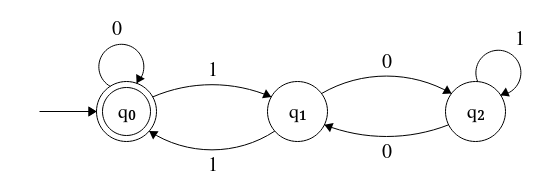
\includegraphics[scale=0.7]{aut1.png}
\end{center}

Este autómata se basa en comprobar que somos congruentes con 0, 1 y 2 con mod 3. 

En el estado $q_0$ simulamos los números congruentes con 0 mod 3 (inicialmente es múltiplo con 3, de ahí que sea estado final), si añadimos un 0, multiplicamos el número por 2, luego sigue siendo congruente con 0 (0 * 2 = 0; 0 mod 3 = 0) (se mantiene en $q_0$), si añadimos un 1, multiplicamos por 2 (sigue siendo congruente con 0) y sumamos 1, así que pasamos a ser congruentes con 1 (0 * 2 = 0; 0 + 1;  1 mod 3 = 1) pasando al estado $q_1$.

En el estado $q_1$ en el que somos congruente con 1 mod 3, si añadimos un 0, multiplicamos por 2, pasando a ser congruentes con 2 (1 * 2 = 2; 2 mod 3 = 2) y al estado $q_2$, si añadimos un 1 multiplicamos por 2 y sumamos 1, pasando a ser congruentes con 0 (1 * 2 = 2; 2 + 1 = 3; 3 mod 3 = 0) de nuevo y pasando al estado $q_0$.


En el estado $q_2$ en el que somos congruente con 2 mod 3 si añadimos un 0, multiplicamos con 2, pasando a ser congruentes con 1 (2*2 = 4; 3 mod 3 = 1) y al estado $q_1$, si añadimos un 1 multiplicamos por 2 y sumamos 1, siguiendo congruentes con 2 mod 3 (2*2 = 4 + 1 = 5; 5 mod 3 = 2) , y permanecemos en $q_2$.



Para la gramática, a partir del autómata determinista obtenemos la siguiente:

\begin{center}

	$$S \rightarrow 0S \vert\ 1S_1 $$
	$$S_1 \rightarrow 0S_2 \vert 1S $$
	$$S_2 \rightarrow 1S_2 \vert 0S_1$$

\end{center}

\newpage

Para conseguir la expresión regular a partir del AFD hacemos que cada estado tenga asociada una ecuación de cambio de estado. Obtenemos las siguientes:

$$ x_0 = 0x_0 + 1x_1 + \epsilon $$
$$ x_1 = 0x_2 + 1x_0$$
$$x_2 = 1x_2 + 0x_1$$

Aplicando que si $x_i = Ax_i + B$ se asocia la expresión regular A*B, de $x_2$ obtenemos: $1$*$0x_1$


Sustituyendo esto en $x_1$ obtenemos que $x_1 = 01$*$0x_1 + 1x_0$ por lo que $x_1 = (01$*$0)$*$1x_0$

Sustituyendo $x_1$ en $x_0$ obtenemos que $x_0 = 0x_0 + 1(01$*$0)$*$1x_0 + \epsilon$, sacando factor común $x_0 = x_0(0 + 1(01$*$0)$*$1) + \epsilon$

Luego $x_0 =(0 + 1(01$*$0)$*$1)$*



\textbf{Ejercicio 2:} Calcular  un  autómata  finito  determinista  que  acepte  el  lenguaje  de  las  palabras  formadas por 0’s y 1’s que empiezan o terminan (o ambas cosas) en 101.

La expresión regular de este autómata sería la siguiente: ( (101)*(0+1)*(101)$^+$) +  ( (101)$^+$(0+1)*(101)* ), es decir, aceptamos las cadenas que tengan como mínimo 101 al final y puedan tener o no tener 101 al principio, o como mínimo 101 al principio o tener 101 o no al final.

\begin{center}
	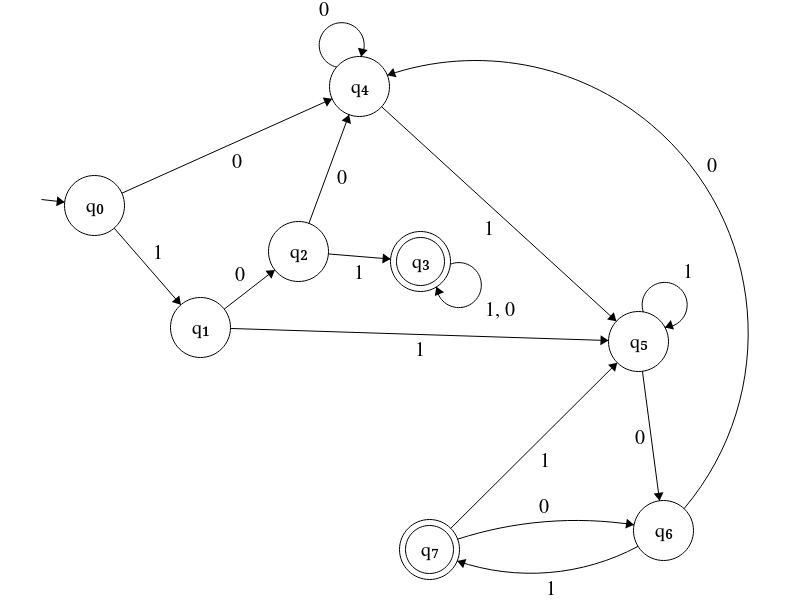
\includegraphics[scale=0.4]{aut2.png}
\end{center}

\newpage

\textbf{Ejercicio 3:} Calcula una máquina de Mealy que codifique secuencias de 0’s y 1’s de la siguiente manera:

\begin{enumerate}
	\item Para cada bit recibido devuelve dos bits.
	\item El primero es la suma (binaria) del bit recibido y de los dos anteriores.
	\item El segundo es la suma (binaria) del bit recibido y el anterior.
	\item Suponemos que los dos bits recibidos antes que el primero son ambos cero.

\end{enumerate}

Cada estado representa los valores de los dos últimos estados. Las salidas serán las sumas, como nos indica el enunciado.

\begin{center}
	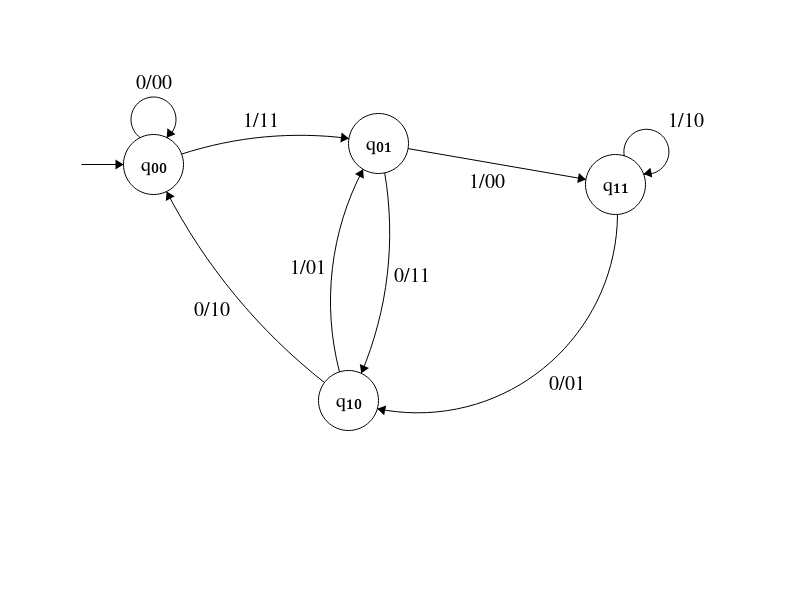
\includegraphics[scale=0.5]{aut3.png}
\end{center}

\newpage

\textbf{Ejercicio 4:} Diseñar una máquina de Mealy o de Moore que, dada una cadena de entrada usando el alfabeto A={a, w, o}, encienda un led verde (salida V) cada vez que se detecte la cadena \texttt{wwow} en la entrada, apagándolo cuando lea cualquier otro símbolo después de esta cadena(representamos el led apagado con la salida X). El autómata tiene que encender el led verde tantas veces como aparezca en la secuencia \texttt{wwow} en la entrada, incluso cuando dos de estas secuencias puedan estar solapadas.

Para este ejercicio crearé una máquina de Moore, en el que al pasar al estado de lectura de la última w devuelvo V, y en otro caso devuelve X.



\begin{center}
	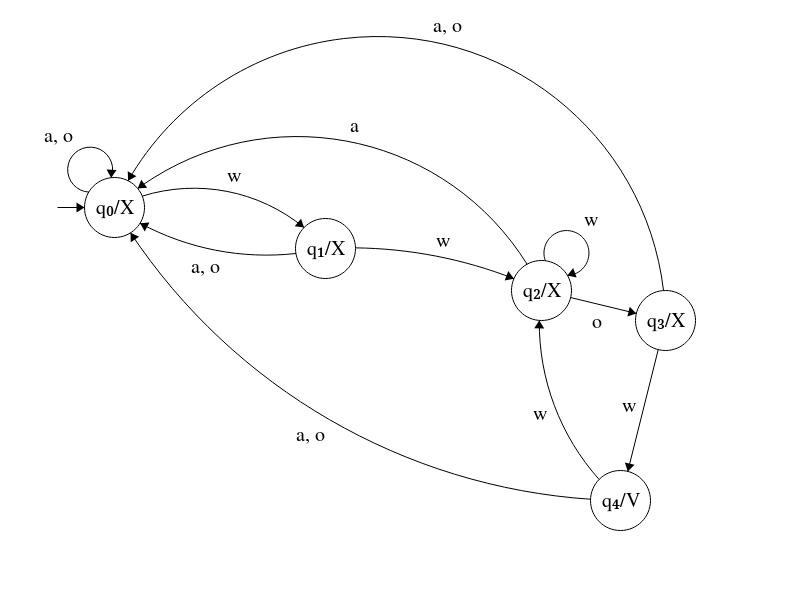
\includegraphics[scale=0.5]{aut4.png}
\end{center}

\end{document}
